
\section{Conclusiones sobre el software utilizado}

Ha sido mucha la diversidad de software (complidores, bibliotecas y herramientas)
utilizado para la realización de este proyecto. Nótese que todo él se ha podido
desarrollar utilizando únicamente \emph{software libre}.

\subsection{Python}

Este proyecto esta desarrollado integramente en Python. Python\footnote{\url{http://www.python.org/}}
se trata de un lenguaje interpretado, orientado a objetos y de tipado dinámico.
Las necesidades del proyecto se han visto sobradamente satisfechas con este lenguaje,
tanto por su eficaz utilización de recursos como por su amplia biblioteca. 

\subsection{Bibliotecas\label{sec:conclu:bib}}

Han sido varias las bibliotecas utilizadas por los distintos componentes software
del proyecto.

\subsubsection{RDFLib}

RDFLib\footnote{\url{http://rdflib.net/}} se trata de una de las bibliotecas
existentes para manejar RDF de forma nativa desde Python. Es parte muy 
importante de SWAML, pues todo el desarrollo se encuentra construido encima 
de esta biblioteca: parseo de RDF, serialización, consultas SPARQL, etc. Aunque 
aún tiene que madurar algunos aspectos, y lo hará dada la activa comunidad de
desarrolladores que hay involucrada, ha sido suficiente para las necesidades
del proyecto.

\subsubsection{mailbox}

El modulo mailbox\footnote{\url{http://docs.python.org/lib/module-mailbox.html}}
sirve para manejar ficheros mbox. Ha jugado un papel importante, pues usarlo
ha permitir al proyecto abstraerse de ese problema para centrarse en los
objetivos que realmente eran importantes.

\subsubsection{ConfigParser}

ConfigParser\footnote{\url{http://docs.python.org/lib/module-ConfigParser.html}}
es un modulo para analizar y abstraer los valores de las configuraciones descritas
en ficheros INI. Los ficheros INI ha sido el mecanismo utilizado en el proyecto
para describir las configuraciones; así pues el correcto funcionamiento de ese 
modulo ha sido importante para el proyecto.

\subsubsection{PyGTK}

PyGTK\footnote{\url{http://pygtk.org/}} provee un wrapper sencillo y eficaz 
para desarrollar interfaces de usuario GTK+\footnote{\url{http://www.gtk.org/}} 
desde Python. En el proyecto se ha usado para el desarrollo de un componente 
muy importante (Buxon) que requeria de una interfaz de usuario gráfica.

\subsubsection{dom.xml}

Con dom.xml\footnote{\url{http://docs.python.org/lib/module-xml.dom.html}} se
provee a Python la capacidad de manejar las funciones básicas del DOM de XML.
Aunque posee muchas más caracteristicas, para lo fines del proyecto sólo
ha sido necesario utilizarlo para la creación de nuevos documentos XML,
desarrollandose una pequeña biblioteca específica para la creación de 
documentos en formato KML.

\subsubsection{Epydoc}

Epydoc\footnote{\url{http://epydoc.sourceforge.net/}} es una herramienta de
generación automática de documentación HTML para Python, al estilo del popular
Javadoc en Java. Ha sido usado para documentar toda la API de proyecto en
la dirección \url{http://swaml.berlios.de/doc/}.

\subsection{Herramientas}

Así mismo han sido innumerables las herramientas utilizadas en distintos para 
aspectos del proyecto. Aquí se pasara a realizar una breve reseña de las más 
destacadas.

\subsubsection{Subversion}

Subversion\footnote{\url{http://subversion.tigris.org/}} es un sistema de 
control de versiones moderno y eficaz de licencia libre. En estos meses se 
han realizado más de 500 commits en el repositorio, por lo que ha sido una
de las herramientas más importantes en todo el ciclo de desarrollo del
proyecto.

\begin{figure}[H]
	\centering
	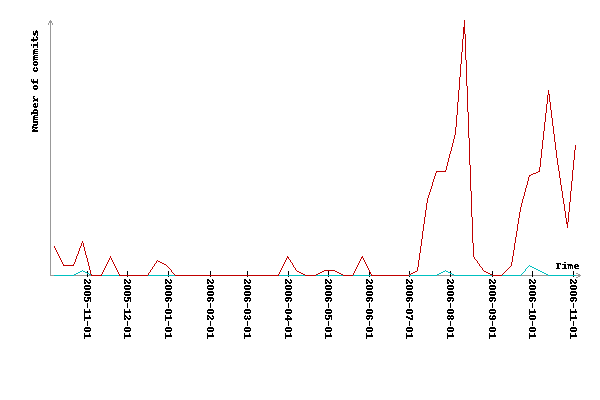
\includegraphics[width=12cm]{images/svn-stats.png}
	\caption{Estadísticas del commits hechos en el subversion de SWAML}
	\label{fig:svnStats}
\end{figure}

\subsubsection{Autotools}

Autotools son un conjunto de herramientas muy extendidas en proyectos de
software libre. En este caso sólo ha sido usado GNU Make\footnote{\url{http://www.gnu.org/software/make/}}
para la automatización de determinas tareas.

\subsubsection{PyDev}

PyDev\footnote{\url{http://pydev.sourceforge.net/}} es un plugin que añade
a Eclipse\footnote{\url{http://eclipse.org/}} la capacidad de desarrolla
Python arpovechando todas las ventajas de este popular IDE.

\subsubsection{Ant}

Ant\footnote{\url{http://ant.apache.org/}} es una herramienta de desarrollo 
similar a la conocida \texttt{make} (y todos sus derivados) que trata de 
superar determinadas deficiencias de esta. Construido en Java sobre XML, 
lo que le aporta una alta capacidad de portabilidad. Utiliza un sistema 
orientado a objetos y extensible para realizar las tareas descritas en un 
fichero llamado \texttt{build.xml}.

El uso de Ant en este proyecto no ha sido ni mucho menos intensivo, apenas para
automatizar determinadas tareas, como por ejemplo transformaciones XSLT.

\subsubsection{Gazpacho}

Gazpacho\footnote{\url{http://gazpacho.sicem.biz/}} es un diseñador de inerfaces
gráficas para la biblioteca de controles de GTK+. Separa el desarrollo de la interfaz
de sus funcionalidad propiamente dicha; para ello genera una descripción en XML
de la interfaz que luego puede ser \emph{cargada} con 
libglade\footnote{\url{http://www.jamesh.id.au/software/libglade/}} para usarse
desde múltiples lenguajes de programación.

\subsubsection{SWOOP}

Existen varios editores libres para ontologías OWL:

\begin{itemize}
  \item Protégé\footnote{\url{http://protege.stanford.edu/plugins/owl/}}
  \item SWeDE\footnote{\url{http://owl-eclipse.projects.semwebcentral.org/}}
  \item SWOOP\footnote{\url{http://www.mindswap.org/2004/SWOOP/}}
\end{itemize}

Los dos primeros no son más que plug-ins para dar soporte a OWL en dos 
frameworks. Y el tercero es un editor pensado y desarrollado explicitamente
para trabajar con OWL.

Después de las pruebas realizadas, SWOOP resultó ser una herramienta más sencilla,
comoda de usar y potente que las otras dos.

\begin{figure}[ht]
	\centering
	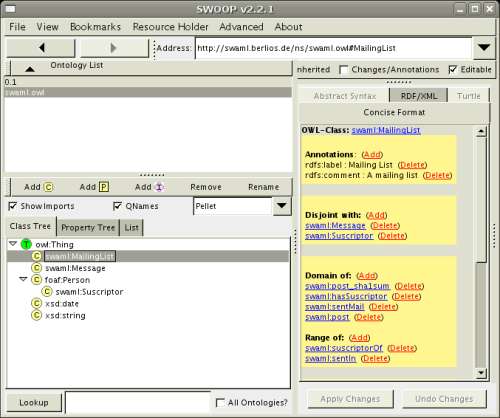
\includegraphics[width=11cm]{images/screenshots/swoop.png}
	\caption{SWOOP editando la ontología de SWAML en OWL DL}
	\label{fig:evoWeb}
\end{figure}

Alguna de las caracteristicas más interesantes de SWOOP son:

\begin{itemize}
  \item Interfaz de usuario hypermedia similar a la de un navegador convencional, 
	con elementos (pestañas, marcadores, etc) que hacen la interfaz más 
	amigable.
  \item Soporte de depuración de la ontología.
  \item Cliente para hacer razonamientos sencillos con Pellet.
\end{itemize}

Un problema común en todas estas herramientas de alto nivel para trabajar con
grafos RDF es el serializado del grafo a sintáxis XML. No por su corrección,
que la herramienta lo hace perfectamente, sino por su orden: es muy difícil
que al serializar queden todos los nodos en el mismo orden. Por tanto es muy
difícil conocer las diferencias entre distintas versiones con las herramientas
convencionales (principalmente \texttt{diff}).

\subsubsection{phpWiki}

phpWiki\footnote{\url{http://phpwiki.sourceforge.net/}} es uno de los wikis
más veteranos. Ha sido usado, sobre todo en etapas tempranas del desarrollo, 
como medio ágil y rápido de documentación colaborativa.

\subsubsection{Umbrello}

Umbrello\footnote{\url{http://uml.sourceforge.net/}} es quizás el editor de
diagramas UML más maduro en la actualidad en el panorama del software libre.
Aunque quizás no esté a la altura de otros editores comerciales, se ha mostrado
una herramienta capaz y suficiente paras las necesidades de este proyecto.

\subsubsection{\LaTeX}

\TeX/\LaTeX es sin duda el sistema de edición de documentos más potente en la
actualidad. La presente documentación ha sido escrita utilizando \LaTeXe con
la ayuda de dos herramientas:

\begin{itemize}
  \item \textbf{Kile\footnote{\url{http://kile.sourceforge.net/}}:} entorno
	integrado para la edición de \LaTeX.
  \item \textbf{JabRef\footnote{\url{http://jabref.sourceforge.net/}}:} aplicación
	para gestionar la bibliografia en formato BibTeX.
\end{itemize}


